\documentclass[12pt]{article}
 \usepackage[margin=1in]{geometry}
\usepackage{amsmath,amsthm,amssymb,amsfonts,listings,color,graphicx}

\newcommand{\N}{\mathbb{N}}
\newcommand{\Z}{\mathbb{Z}}
\definecolor{mygreen}{RGB}{28,172,0} % color values Red, Green, Blue
\definecolor{mylilas}{RGB}{170,55,241}

\newenvironment{problem}[2][Problem]{\begin{trivlist}
\item[\hskip \labelsep {\bfseries #1}\hskip \labelsep {\bfseries #2.}]}{\end{trivlist}}
%If you want to title your bold things something different just make another thing exactly like this but replace "problem" with the name of the thing you want, like theorem or lemma or whatever

\begin{document}
\lstset{language=Matlab,%
    %basicstyle=\color{red},
    breaklines=true,%
    morekeywords={matlab2tikz},
    keywordstyle=\color{blue},%
    morekeywords=[2]{1}, keywordstyle=[2]{\color{black}},
    identifierstyle=\color{black},%
    stringstyle=\color{mylilas},
    commentstyle=\color{mygreen},%
    showstringspaces=false,%without this there will be a symbol in the places where there is a space
    numbers=left,%
    numberstyle={\tiny \color{black}},% size of the numbers
    numbersep=9pt, % this defines how far the numbers are from the text
    emph=[1]{for,end,break},emphstyle=[1]\color{red}, %some words to emphasise
    %emph=[2]{word1,word2}, emphstyle=[2]{style},
}





\title{Econ 675: HW 1}
\author{Erin Markiewitz}
\maketitle
\newpage
\tableofcontents


\section{Simple Linear Regression w/ Measurement Error}
\subsection{}



 By LLN,
\begin{equation}
\begin{split}
\hat{\beta_{LS}} & = \frac{\mathbf{\tilde{x}'x}}{\mathbf{\tilde{x}'\tilde{x}}}\beta  +  \frac{\mathbf{\tilde{x}'\epsilon}}{\mathbf{\tilde{x}'x}} = \frac{\mathbf{\tilde{x}'x/}n}{\mathbf{\tilde{x}'\tilde{x}/}n}\beta  +  \frac{\mathbf{\tilde{x}'\epsilon/}n}{\mathbf{\tilde{x}'x}/n} \\
& \rightarrow_p  \frac{\mathop{\mathbb{E}}[ (x_i + u_i)x_i ]}{\mathop{\mathbb{E}}[(x_i + u_i)^2]}\beta = \frac{\sigma_x^2}{\sigma_x^2 + \sigma_u^2} \beta = \lambda\beta
 \end{split}
 \end{equation}

 As $\sigma_x^2, \sigma_u^2 > 0 \implies \frac{\sigma_x^2}{\sigma_x^2 + \sigma_u^2} < 1, \lambda\beta < \beta$.   $\hat{\beta}_{LS}$ is biased downward.


 \subsection{}



By LLN,
\begin{equation}
\begin{split}
\hat{\sigma}_\epsilon^2 & = (\mathbf{y - (x+u)}(\hat{\beta}_{LS} )' (\mathbf{y - (x+u)}(\hat{\beta}_{LS} )/n \\
& = (\mathbf{\epsilon} - (\hat{\beta}_{LS} - \beta)\mathbf{x} - \mathbf{u}\hat{\beta}_{LS})'(\mathbf{\epsilon} - (\hat{\beta}_{LS} - \beta)\mathbf{x} - \mathbf{u}\hat{\beta}_{LS})/n\\
&= \mathbf{\epsilon}'\mathbf{\epsilon}/n - (\hat{\beta}_{LS} - \beta)\mathbf{\epsilon}'\mathbf{x}/n -\mathbf{\epsilon}'\mathbf{u}/n \\
&+ (\hat{\beta}_{LS} - \beta)\mathbf{x}'\mathbf{\epsilon}/n + (\hat{\beta}_{LS} - \beta)^2\mathbf{x}'\mathbf{x}/n  \\
&+ (\hat{\beta}_{LS} - \beta)\hat{\beta}_{LS}\mathbf{x}'\mathbf{u}/n+\hat{\beta}_{LS}\mathbf{x}'\mathbf{\epsilon}/n + \beta)\hat{\beta}_{LS}\mathbf{u}'\mathbf{x}/n +\hat{\beta}_{LS}^2\mathbf{u}'\mathbf{u}/n \\
&\rightarrow_p \sigma_\epsilon^2 +o_p(1) + o_p(1) + o_p(1) +(1-\lambda)^2\beta^2\sigma_x^2+o_p(1)+o_p(1)+o_p(1)+\lambda^2\beta^2\sigma_u^2\\
&=  \sigma_\epsilon^2 +(1-\lambda)^2\beta^2\sigma_x^2+\lambda^2\beta^2\sigma_u^2
 \end{split}
 \end{equation}
 which has an upward bias.


Now considering $\sigma_\epsilon^2(\mathbf{\tilde{x}'\tilde{x}}/n)^{-1}$ using our previous results,
\begin{equation}
\begin{split}
\sigma_\epsilon^2(\mathbf{\tilde{x}'\tilde{x}}/n)^{-1} &\rightarrow_p  \frac{\sigma_\epsilon^2 +(1-\lambda)^2\beta^2\sigma_x^2+\lambda^2\beta^2\sigma_u^2}{\sigma_x^2+\sigma_u^2} = \lambda\frac{\sigma_\epsilon^2}{\sigma_x^2} + \lambda(1-\lambda)\beta^2
 \end{split}
 \end{equation}

We cannot sign the bias with the information provide.
\newpage
\subsection{}


By Slutsky and previous results,

\begin{equation}
\begin{split}
\frac{\hat{\beta}_{LS}}{\sqrt{\sigma_\epsilon^2(\mathbf{\tilde{x}'\tilde{x}}/n)^{-1}}} &\rightarrow_p \frac{\sqrt\lambda\beta}{\sqrt{\frac{\sigma_\epsilon^2}{\sigma_x^2} + (1-\lambda)\beta^2}}
 \end{split}
 \end{equation}

\begin{equation}
\begin{split}
\frac{\sqrt\lambda\beta}{\sqrt{\frac{\sigma_\epsilon^2}{\sigma_x^2} + (1-\lambda)\beta^2}} < \frac{\beta}{\sqrt{\frac{\sigma_\epsilon^2}{\sigma_x^2}}}
 \end{split}
 \end{equation}

 So the estimate is biased downward.


 \subsection{}


As the instrument is uncorrelated with $u_i$ and $\epsilon_i$,

\begin{equation}
\begin{split}
\hat{\beta}_{IV} & = \frac{\mathbf{\check{x}'y}}{\mathbf{\check{x}'\tilde{x}}}  = \frac{\mathbf{\check{x}'y}/n}{\mathbf{\check{x}'\tilde{x}}/n}\beta  +  \frac{\mathbf{\check{x}'\epsilon}/n}{\mathbf{\check{x}'\tilde{x}}/n} \rightarrow_p
\frac{\mathop{\mathbb{E}}[\check{x_i} x_i ]}{\mathop{\mathbb{E}}[\check{x}_i(x_i + u_i)]}\beta = \beta
\end{split}
\end{equation}

\subsection{}

$ \mathbf{y} = \mathbf{x}\beta + \mathbf{\epsilon} =  \mathbf{(\tilde{x} - u)}\beta + \mathbf{\epsilon}
=  \mathbf{\tilde{x}}\beta + (\mathbf{\epsilon- u}\beta) $



\begin{equation}
\begin{split}
\sqrt{n}(\hat{\beta}_{IV}  - \beta) & = \sqrt{n}\left(\frac{\mathbf{\check{x}'\tilde{x}}}{\mathbf{\check{x}'\tilde{x}}}\beta
+ \frac{\mathbf{\check{x}'(\epsilon- u}\beta)}{\mathbf{\check{x}'\tilde{x}}} - \beta\right) \\
& = \frac{\mathbf{\check{x}'(\epsilon- u}\beta)/\sqrt{n}}{\mathbf{\check{x}'\tilde{x}}/n}
= (\mathop{\mathbb{E}}[\check{x}_i x_i])^{-1} \frac{\mathbf{\check{x}'(\epsilon- u}\beta)}{\sqrt{n}} +o_p(1) \rightarrow_d N(0,V_{IV})
\end{split}
\end{equation}

where $V_{IV} = \frac{\mathop{\mathbb{E}}[\check{x}_i^2(\epsilon_i- u_i\beta)^2]}{(\mathop{\mathbb{E}}[\check{x}_i x_i])^2}   $




\subsection{}


First, estimate heteroskedasticity-consistent standard errors:
\begin{equation}
\begin{split}
  \hat{V}_{IV} & = \left(\frac{\mathbf{\check{x}'\tilde{x}}}{n}\right)^{-1} \left(\frac{1}{n}\sum^n_{i=1}\check{x}_i^2(y_i-\check{x}_i\hat{\beta}_{IV})^2\right) \left(\frac{\mathbf{\check{x}'\tilde{x}}}{n}\right)^{-1}
   = \frac{\mathop{\mathbb{E}}[\check{x}_i^2(\epsilon_i- u_i\beta)^2]}{(\mathop{\mathbb{E}}[\check{x}_i x_i])^2} +o_p(1) \\
   & \rightarrow_p V_{IV}
\end{split}
\end{equation}


Then, construct the confidence interval

\begin{equation}
\begin{split}
  CI_{95} = \left[\hat{\beta}_{IV}  \pm 1.96 * \sqrt{\frac{\hat{V}_{IV}}{n}}\right]
\end{split}
\end{equation}

\newpage

\subsection{}

From 1.1 we know $ \hat{\lambda} = \frac{\mathbf{\check{\sigma}_x^2}}{\mathbf{\tilde{x}'\tilde{x}}} \rightarrow_p \frac{\sigma_x^2}{\sigma_x^2 + \sigma_u^2} = \lambda $, so $\frac{\hat{\beta}_{IV}}{\hat{\lambda}} \rightarrow_p \beta$

\subsection{}


Define the function $g(w) = w_1w_2/w_3$ where $\mathbf{w} = (w_1, w_2, w_3)\in\mathbb{R}$ such that $\mathbf{\dot{g}(w)} = (w_2/w_3,w_1/w_3,-w_1w_2/w_3^2)$. By the delta method.

\begin{equation}
\begin{split}
  \sqrt{n} \left( g \left(
\begin{bmatrix}
\hat{\beta}_{LS} \\
\mathbf{\tilde{x}'\tilde{x}}/n \\
\mathbf{\check{\sigma}_x^2} \\
\end{bmatrix}
\right)  - g \left(
\begin{bmatrix}
\lambda \beta \\
\mathbf{\sigma_x^2 + \sigma_u^2} \\
\mathbf{\sigma_x^2} \\
\end{bmatrix} \right) \right)
= \sqrt{n}\left(\frac{\hat{\beta}_{IV}}{\hat{\lambda}} - \beta\right) \rightarrow_d N(0,V_{VS})
\end{split}
\end{equation}

where $V_{VS} = \mathbf{\dot{g}(w_0)}' \Sigma \mathbf{\dot{g}(w_0)}$ and
$ \mathbf{w_0} = (\lambda\beta,\sigma_x^2 + \sigma_u^2,\sigma_x^2)$

\subsection{}

Assuming there is an estimator $\hat{\Sigma}$,
\begin{equation}
\begin{split}
  CI_{95} = \left[\mathbf{g(\hat{w})} \pm 1.96 * \sqrt{\frac{\hat{V}_{VS}}{n}}\right]
\end{split}
\end{equation}

  where $V_{VS} = \mathbf{\dot{g}(\hat{w})}' \hat{\Sigma} \mathbf{\dot{g}(\hat{w})} $
  and
  $\mathbf{\hat{w}} = (\hat{\beta}_{LS}, \mathbf{\tilde{x}'\tilde{x}}/n  ,\check{\sigma}_x^2)$


  \subsection{}


The fixed effects estimator is equivalent to the first differences estimator when t=2:
$\hat{\beta}_{FE} = \mathbf{\frac{\Delta\tilde{x}\Delta y}{\Delta\tilde{x}\Delta\tilde{x}}}$
where $\mathbf{\Delta\tilde{x} = \tilde{x}_2 - \tilde{x}_1}$ and $\mathbf{\Delta y = y_2 - y_1}$. Note,  $\Delta y_i = (\Delta x_i - \Delta u_i)\beta + \Delta\epsilon_i$ where $\epsilon_i = \epsilon_{i2} - \epsilon_{i1} $

\begin{equation}
\begin{split}
\hat{\beta}_{FE} = \mathbf{\frac{\Delta\tilde{x}\Delta y}{\Delta\tilde{x}\Delta\tilde{x}}} \rightarrow_p \mathbf{\frac{\mathop{\mathbb{E}}[(\Delta x_i + \Delta u_i)\Delta x_i]}{\mathop{\mathbb{E}}[(\Delta x_i + \Delta u_i)^2]}}\beta = \frac{\sigma_{\Delta x}^2}{\sigma_{\Delta x}^2 + \sigma_{\Delta u}^2} = \gamma\beta
\end{split}
\end{equation}

By construction $\gamma<1$, therefore $\hat{\beta}_{FE}$ is biased downward.


\subsection{}

Using the previous result

\begin{equation}
\begin{split}
\gamma & = \frac{\sigma_{\Delta x}^2}{\sigma_{\Delta x}^2 + \sigma_{\Delta u}^2} =
\frac{\mathop{\mathbb{V}}[x_{i2} - x_{i1}]}{\mathop{\mathbb{V}}[x_{i2} - x_{i1}] + \mathop{\mathbb{V}}[u_{i2} - u_{i1}]} = \frac{2\sigma_x^2 -2 \mathop{\mathbb{C}}[x_{i2},x_{i1}]}{2\sigma_x^2 -2  \mathop{\mathbb{C}}[x_{i2},x_{i1}] + 2\sigma_u^2 -2 \mathop{\mathbb{C}}[u_{i2},u_{i1}]} \\
& = \frac{\sigma_x^2(1-\rho_x)}{\sigma_x^2(1-\rho_x) + \sigma_u^2(1-\rho_u)} = \frac{\sigma_x^2}{\sigma_x^2 + \sigma_u^2\frac{(1-\rho_u)}{(1-\rho_x)}}
\end{split}
\end{equation}


\subsection{}
If $\rho_x \approx 1$ and $\rho_u \approx 0$, then $\gamma \approx 0$  and $\gamma = \frac{\sigma_x^2}{\sigma_x^2 + \sigma_u^2\frac{(1-\rho_u)}{(1-\rho_x)}} < \frac{\sigma_x^2}{\sigma_x^2 + \sigma_u^2} = \lambda $. Intuitively, if regressors are highly correlated and measurement error is uncorrelated over time, then fixed-effects estimation will produced more biased estimates than simple linear regression.


\section{Implementing Least-Squares Estimators}
\subsection{}

Given the Estimator:
$\mathbf{\hat{\beta}(W)} = argmin_{\beta \ in \mathop{\mathbb{R}}^d} (\mathbf{(y-X\beta)'W(y-X\beta)')}$ Take the FOC.

\begin{equation}
\begin{split}
\mathbf{-X'W(y-X\beta)-(y-X\beta)'WX} & = 0 \\
\mathbf{-X'Wy + X'WX\beta + X'WX\beta - X'Wy} & = 0 \\
\mathbf{ 2X'WX\beta}  & = 2X'Wy  \\
\mathbf{\hat{\beta}(W)} & = \mathbf{(X'WX)^{-1} X'Wy} \\
\end{split}
\end{equation}

\subsection{}

\begin{equation}
\begin{split}
\sqrt{n}\left(\mathbf{\hat{\beta}(W)} - \beta \right) & = \sqrt{n}\left( \mathbf{(X'WX)^{-1} X'W(x_i'\beta + \epsilon)} - \beta \right) \\
& = \left( \mathbf{\beta + \frac{X'W\epsilon/\sqrt{n}}{(X'WX)/n}} - \beta \right)  \\
& = \mathbf{\frac{X'W\epsilon/\sqrt{n}}{(X'WX)/n}} \\
&\rightarrow_d \mathop{\mathbb{V}}(0,\mathbf{V(W)})\
\end{split}
\end{equation}


\hspace{3cm} where $\mathbf{V(W) = (X'WX)^{-1}(X'W\Sigma^{-1}WX)(X'WX)^{-1}}$

Now if $\mathop{\mathbb{V}}\mathbf{[y|X,W] = \sigma^2I_n}$, the sandwich matrix form of $\mathbf{V(W)}$ simplifies:

$\mathbf{V(W) = (X'WX)^{-1}(X'W\sigma^2WX)(X'WX)^{-1} = (X'X)^{-1}\sigma^2 } $

\subsection{}

The following estimator is a consistent variance-covariance estimator of $\mathbf{V(W)}$:

\begin{equation}
\mathbf{\hat{V}(W) = (X'WX) }/n)^{-1} (\mathbf{X'W\epsilon'\epsilon WX}/\sqrt{n})(\mathbf{X'WX}/n)^{-1}
\end{equation}

\subsection{}
 Stata and R code for question 2.4 is in the code appendix

\subsection{}

\subsubsection{}

\begin{center}

R code: Regression Table (matrix)
\par
\begin{tabular}{lrrrr}
  \hline
term & estimate & std.error & statistic & p.value \\
  \hline
(Intercept) & 6485.553 & 4513.513 & 1.437 & 0.151 \\
  treat & 1535.482 & 638.238 & 2.406 & 0.017 \\
  black & -2592.377 & 794.999 & -3.261 & 0.001 \\
  age & 39.341 & 40.470 & 0.972 & 0.332 \\
  educ & -740.540 & 944.679 & -0.784 & 0.434 \\
  educ\_sq & 60.082 & 53.768 & 1.117 & 0.264 \\
  earn74 & -0.030 & 0.104 & -0.288 & 0.774 \\
  black\_earn74 & 0.175 & 0.132 & 1.330 & 0.184 \\
  u74 & 1316.032 & 1505.927 & 0.874 & 0.383 \\
  u75 & -1167.688 & 1275.416 & -0.916 & 0.360 \\
   \hline
\end{tabular}
\par



Stata code: Regression Table (matrix)
\par
\begin{tabular}{lrrrrrr}
  \hline
term & estimate & std.error & statistic & p.value & CI minus &  CI plus \\
  \hline
  treat &  1535.4824 & 638.2380 & 2.4058 & 0.0166 & 281.0688 & 2789.8961 \\
black &  -2592.3766 & 794.9991 & -3.2609 & 0.0012 & -4154.8937 & -1029.8595 \\
  age & 39.3405 & 40.4701 & 0.9721 & 0.3315 & -40.2007 & 118.8817 \\
  educ & -740.5400 & 944.6787 & -0.7839 & 0.4335 & -2597.2421 & 1116.1622 \\
  educ\_sq & 60.0823 & 53.7684 & 1.1174 & 0.2644 & -45.5958 & 165.7604 \\
earn74 & -0.0299 & 0.1037 & -0.2879 & 0.7735 & -0.2337 & 0.1740 \\
  black\_earn74 &  0.1754 & 0.1318 & 1.3304 & 0.1841 & -0.0837 & 0.4344 \\
  u74 & 1316.0320 & 1505.9270 & 0.8739 & 0.3827 & -1643.7657 & 4275.8296 \\
  u75 & -1167.6884 & 1275.4156 & -0.9155 & 0.3604 & -3674.4316 & 1339.0548 \\
(Intercept) & 6485.5531 & 4513.5125 & 1.4369 & 0.1515 & -2385.4508 & 15356.5570 \\
\hline
\end{tabular}
\end{center}

The coefficients match up.

\subsubsection{}
\begin{center}
  R code: Regression Table
  \par
  % latex table generated in R 3.5.1 by xtable 1.8-3 package
% Sun Oct  7 20:42:04 2018
\begin{tabular}{lrrrrrr}
  \hline
variable & beta & se & t\_test & p\_value & CI\_L & CI\_U \\ 
  \hline
const & 6485.55 & 4513.51 & 1.44 & 0.15 & -2384.89 & 15356.00 \\ 
  treat & 1535.48 & 638.24 & 2.41 & 0.02 & 281.15 & 2789.82 \\ 
  black & -2592.38 & 795.00 & -3.26 & 0.00 & -4154.80 & -1029.96 \\ 
  age & 39.34 & 40.47 & 0.97 & 0.33 & -40.20 & 118.88 \\ 
  educ & -740.54 & 944.68 & -0.78 & 0.43 & -2597.13 & 1116.05 \\ 
  educ\_sq & 60.08 & 53.77 & 1.12 & 0.26 & -45.59 & 165.75 \\ 
  earn74 & -0.03 & 0.10 & -0.29 & 0.77 & -0.23 & 0.17 \\ 
  black\_earn74 & 0.18 & 0.13 & 1.33 & 0.18 & -0.08 & 0.43 \\ 
  u74 & 1316.03 & 1505.93 & 0.87 & 0.38 & -1643.58 & 4275.64 \\ 
  u75 & -1167.69 & 1275.42 & -0.92 & 0.36 & -3674.27 & 1338.90 \\ 
   \hline
\end{tabular}

  \newpage
  \par
  Stata Code: Regression Table
  \par
  {
\def\sym#1{\ifmmode^{#1}\else\(^{#1}\)\fi}
\begin{tabular}{l*{1}{c}}
\hline\hline
            &\multicolumn{1}{c}{(1)}\\
            &\multicolumn{1}{c}{earn78}\\
\hline
treat       &      1535.5\sym{*}  \\
            &      (2.41)         \\
[1em]
black       &     -2592.4\sym{**} \\
            &     (-3.26)         \\
[1em]
age         &       39.34         \\
            &      (0.97)         \\
[1em]
educ        &      -740.5         \\
            &     (-0.78)         \\
[1em]
educ2       &       60.08         \\
            &      (1.12)         \\
[1em]
earn74      &     -0.0299         \\
            &     (-0.29)         \\
[1em]
blacke74    &       0.175         \\
            &      (1.33)         \\
[1em]
u74         &      1316.0         \\
            &      (0.87)         \\
[1em]
u75         &     -1167.7         \\
            &     (-0.92)         \\
[1em]
cons        &      6485.6         \\
            &      (1.44)         \\
\hline
\(N\)       &         445         \\
\hline\hline
\multicolumn{2}{l}{\footnotesize \textit{t} statistics in parentheses}\\
\multicolumn{2}{l}{\footnotesize \sym{*} \(p<0.05\), \sym{**} \(p<0.01\), \sym{***} \(p<0.001\)}\\
\end{tabular}
}

\end{center}
The coefficients match up.
\newpage

\section{Analysis of Experiments}
\subsection{}
\subsubsection{}
\begin{equation}
\begin{split}
\mathop{\mathbb{E}}[T_{DM}] & = \mathop{\mathbb{E}}[\bar{Y}_1] - \mathop{\mathbb{E}}[\bar{Y}_0] \\
& = \mathop{\mathbb{E}}[\frac{1}{N_1} \sum_{i=1}^{n} D_i (1) Y_i] - \mathop{\mathbb{E}}[\frac{1}{n - N_1} \sum_{i=1}^{n} D_i (0) Y_i] \\
 & = \mathop{\mathbb{E}}[\frac{1}{N_1} \sum_{i=1}^{n} D_i(1)Y_i(1)] - \mathop{\mathbb{E}}[\frac{1}{n-N_1} \sum_{i=1}^{n}D_i(0)Y_i(0)] \\
 & = \mathop{\mathbb{E}}[\mathop{\mathbb{E}}[\frac{1}{N_1} \sum_{i=1}^{n} D_i(1)Y_i(1)|T_i]] - \mathop{\mathbb{E}}[\mathop{\mathbb{E}}[\frac{1}{n-N_1} \sum_{i=1}^{n} D_i(0)Y_i(0)]|T_i]] \\
 & = \mathop{\mathbb{E}}[\frac{1}{N_1} \sum_{i=1}^{n} \left( \frac{N_1}{n} \right)    Y_i(1)] - \mathop{\mathbb{E}}[\frac{1}{n-N_1} \sum_{i=1}^{n}    \left( \frac{N_1}{n} \right) Y_i(0)] \\
 & = \mathop{\mathbb{E}}[\frac{1}{N_1} \sum_{i=1}^{n} \left( \frac{N_1}{n} \right)    Y_i(1)] - \mathop{\mathbb{E}}[\frac{1}{n-N_1} \sum_{i=1}^{n}    \left( \frac{n- N_1}{n} \right) Y_i(0)] \\
  & = \mathop{\mathbb{E}}[\frac{1}{n} \sum_{i=1}^{n}Y_i(1)] - \mathop{\mathbb{E}}[\frac{1}{n} \sum_{i=1}^{n} Y_i(0)] \\
    & = \frac{1}{n} \sum_{i=1}^{n}Y_i(1) - \frac{1}{n} \sum_{i=1}^{n} Y_i(0)\\
\end{split}
\end{equation}

\subsubsection{}


\begin{center}
  R code: Asymptotically Conservative 95 CI for average treatment effect
  \par
% latex table generated in R 3.5.1 by xtable 1.8-3 package
% Sun Oct  7 20:42:04 2018
\begin{tabular}{rrrr}
  \hline
TDM est & Conservative SE & CI Lower & CI Upper \\ 
  \hline
1794.34 & 671.00 & 479.21 & 3109.47 \\ 
   \hline
\end{tabular}

\end{center}


\begin{center}
  Stata code: Asymptotically Conservative 95 CI for average treatment effect
\par
\begin{tabular}{rrrr}
  \hline
TDM est & Conservative SE & CI Lower & CI Upper \\
1794.3431 & 670.9967 & 479.2137 & 3109.4725 \\
\hline
\end{tabular}
\end{center}

The point estimates, standard errors, and confidence intervals match up across platforms.

\subsection{}

\newpage
\subsubsection{}


\begin{center}
  R code: Sharp Null Hypothesis of No Treatment Effect
  \par
% latex table generated in R 3.5.1 by xtable 1.8-3 package
% Sun Oct  7 20:42:04 2018
\begin{tabular}{r}
  \hline
DM P value \\ 
  \hline
0.01 \\ 
   \hline
\end{tabular}

% latex table generated in R 3.5.1 by xtable 1.8-3 package
% Sun Oct  7 20:42:04 2018
\begin{tabular}{r}
  \hline
KS P value \\ 
  \hline
0.03 \\ 
   \hline
\end{tabular}

\par
Stata Code: Sharp Null Hypothesis of No Treatment Effect
\par

\begin{tabular}{rr}
  \hline
DM P value & KS P Value\\
  \hline
.0045 & .034\\
   \hline
\end{tabular}

\end{center}


The p-values line up for the most part. The differences are rounding errors.

\subsubsection{}
\begin{center}
Stata Code: Finite Sample valid 95 CI for the treatment effect
\par
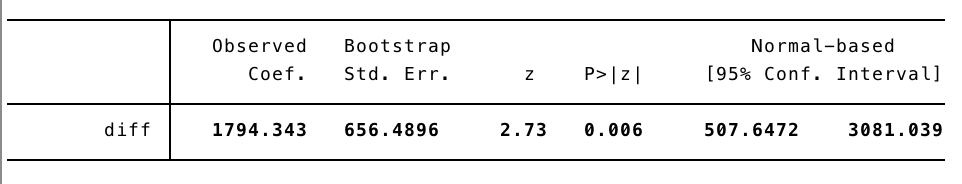
\includegraphics[totalheight=2cm]{stata_table}
\par
R Code: Finite Sample valid 95 CI for the treatment effect
\par
\tiny

% latex table generated in R 3.5.1 by xtable 1.8-3 package
% Sun Oct  7 20:42:04 2018
\begin{tabular}{rr}
  \hline
Hypothesized Treatment Effect & p\_value \\ 
  \hline
5000.00 & 0.00 \\ 
  4750.00 & 0.00 \\ 
  4500.00 & 0.00 \\ 
  4250.00 & 0.00 \\ 
  4000.00 & 0.00 \\ 
  3750.00 & 0.00 \\ 
  3500.00 & 0.01 \\ 
  3250.00 & 0.02 \\ 
  3000.00 & 0.04 \\ 
  2750.00 & 0.10 \\ 
  2500.00 & 0.29 \\ 
  2250.00 & 0.50 \\ 
  2000.00 & 0.76 \\ 
  1750.00 & 0.94 \\ 
  1500.00 & 0.65 \\ 
  1250.00 & 0.39 \\ 
  1000.00 & 0.21 \\ 
  750.00 & 0.11 \\ 
  500.00 & 0.05 \\ 
  250.00 & 0.01 \\ 
  0.00 & 0.01 \\ 
  -250.00 & 0.00 \\ 
  -500.00 & 0.00 \\ 
  -750.00 & 0.00 \\ 
  -1000.00 & 0.00 \\ 
  -1250.00 & 0.00 \\ 
  -1500.00 & 0.00 \\ 
   \hline
\end{tabular}

\normalsize

\end{center}
The confidence intervals match up across platforms. The Rubin's technique of bootstrapping the p-value was easier to implement the question in R. Looking at the table from R, it is clear that the confidence interval from Stata is congruent.

\newpage
\subsection{}
\subsubsection{}
\begin{center}
  Stata: Power Function
  \par
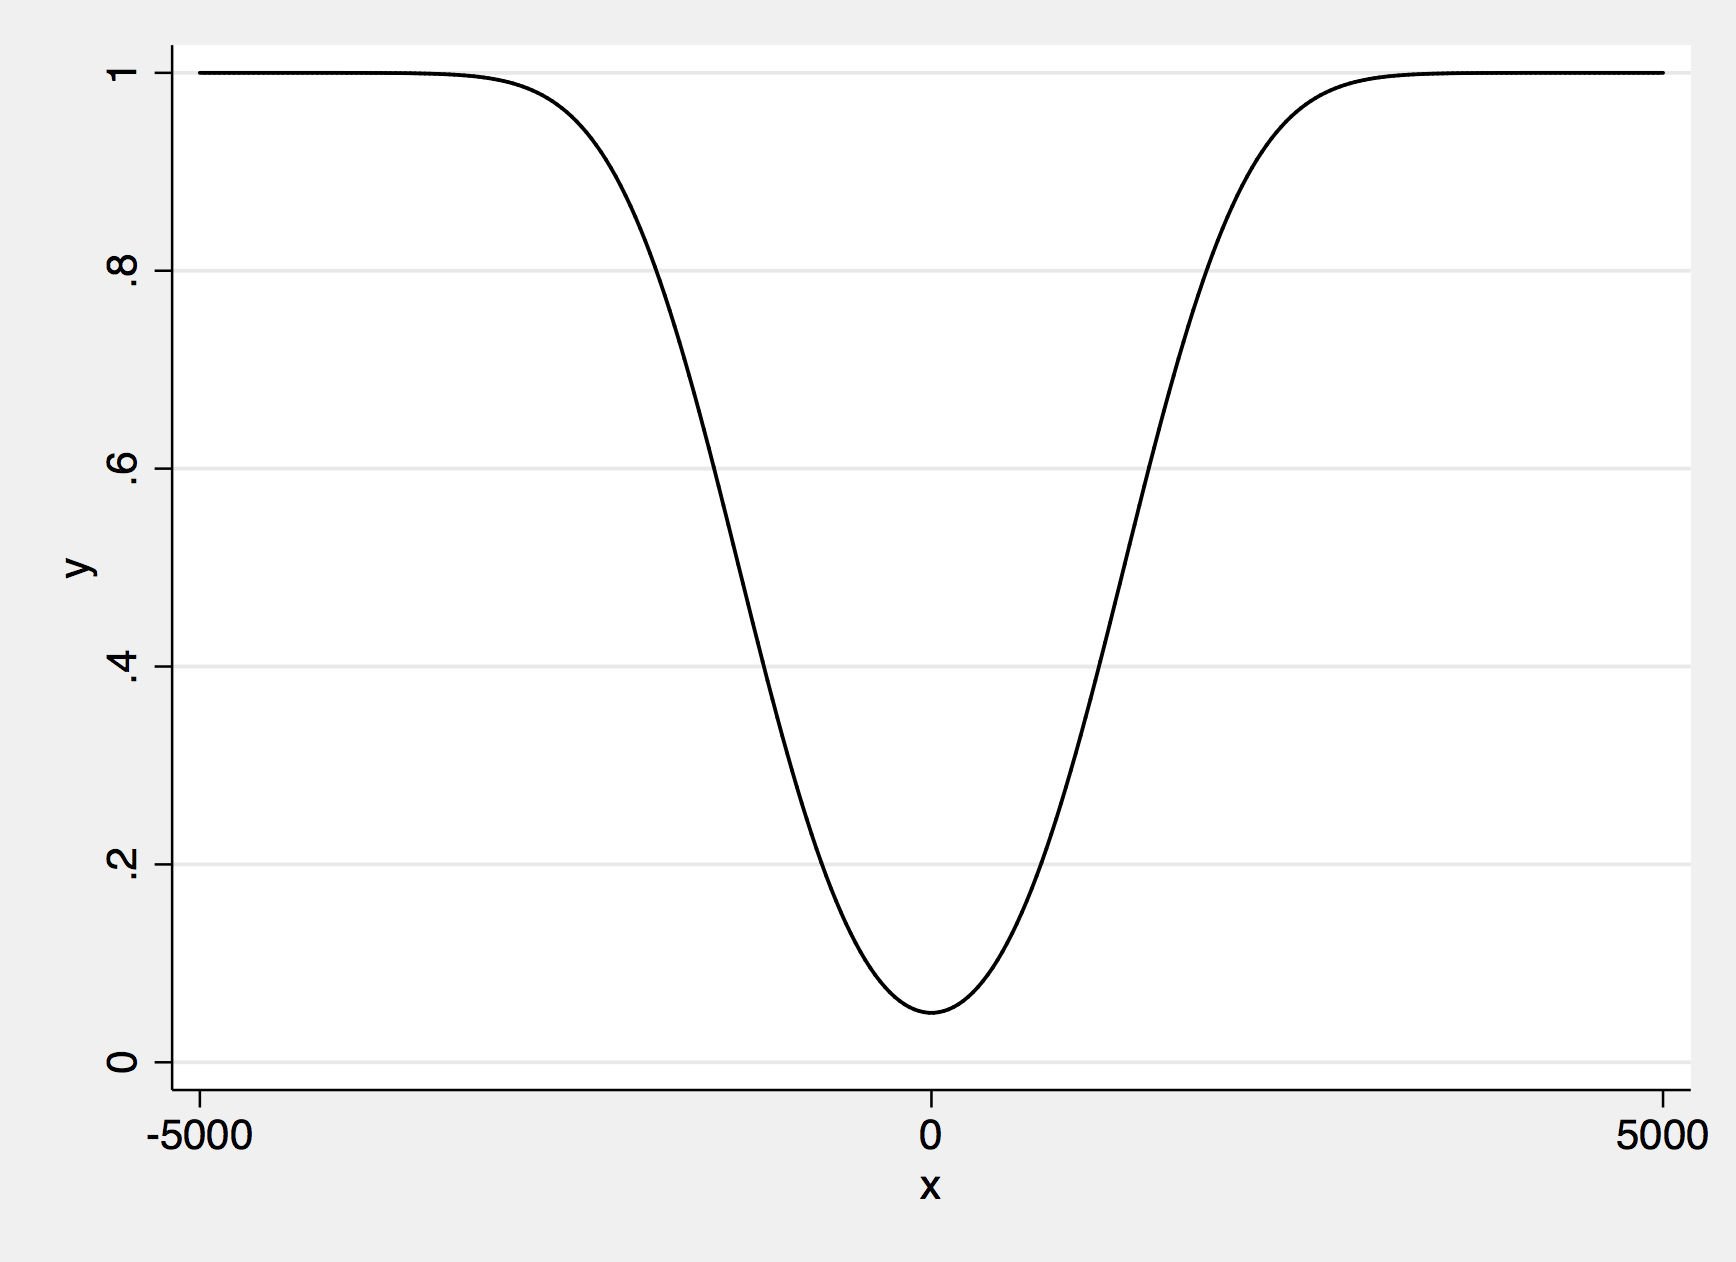
\includegraphics[totalheight=8cm]{stata_power.png}
\par
R: Power Function
\par
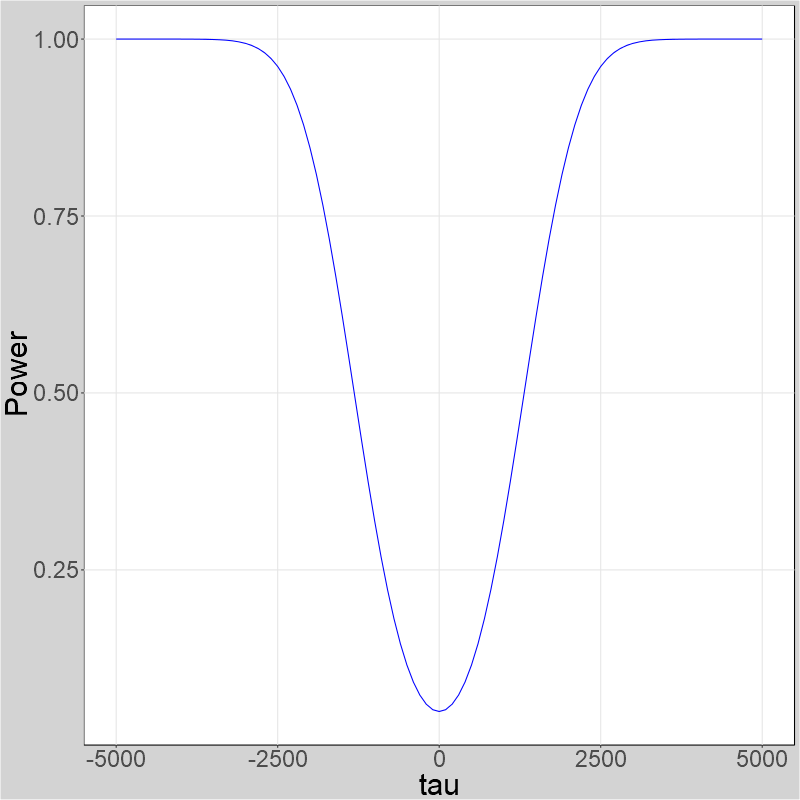
\includegraphics[totalheight=8cm]{power_func_r.png}
\end{center}


\subsubsection{}

  Stata computes that the sufficient sample size: 1436.824051\\
  R computes that the sufficient sample size:  1436.824

  The difference is clearly a rounding error.

\begin{center}
\end{center}


\begin{center}


\end{center}

\section{Code Appendix}
\subsection*{Stata}
\lstinputlisting{econ675hw1.do}
\subsection*{R}
\lstinputlisting{econ675_hw1.R}
\end{document}
